\documentclass{beamer}
\usepackage[utf8]{inputenc}

\usetheme{Madrid}
\usecolortheme{default}
\usepackage{amsmath,amssymb,amsfonts,amsthm}
\usepackage{txfonts}
\usepackage{tkz-euclide}
\usepackage{listings}
\usepackage{gvv}
\usepackage{graphicx}

% Setup for code listings
\lstset{
    language=C,
    basicstyle=\ttfamily\small,
    keywordstyle=\color{blue},
    stringstyle=\color{orange},
    commentstyle=\color{green!60!black},
    numbers=left,
    numberstyle=\tiny\color{gray},
    breaklines=true,
    showstringspaces=false,
}
%------------------------------------------------------------
% Title page information
\title{1.5.4}
\author{Taraka Abhinav - EE25BTECH11016}
\date{\today}
%------------------------------------------------------------

\begin{document}

\frame{\titlepage}

\begin{frame}{Question}
A circle has its center at $(4, 4)$. If one end of a diameter is $(4, 0)$, then find the coordinates of the other end.
\end{frame}

\begin{frame}{Theoretical Solution}
Let the position vectors for the center, the known end, and the unknown end of the diameter be $\vec{C}$, $\vec{B}$, and $\vec{A}$ respectively. Let the coordinates of the unknown end $\vec{A}$ be $(a,b)$.

The given vectors are:
\begin{align}
\vec{A} = \myvec{a\\b}, \quad \vec{B} = \myvec{4\\0}, \quad \vec{C} = \myvec{4\\4}
\end{align}

The center of the circle is the midpoint of the diameter. Therefore, the center vector is the average of the endpoint vectors.
\begin{align}
\vec{C} = \frac{\vec{A}+\vec{B}}{2}
\end{align}

To find the unknown vector $\vec{A}$, we rearrange the equation:
\begin{align}
2\vec{C} &= \vec{A} + \vec{B} \\
\vec{A} &= 2\vec{C} - \vec{B}
\end{align}

\end{frame}

\begin{frame}{Theoretical Solution}
Substituting the given vector values:
\begin{align}
\myvec{a\\b} &= 2\myvec{4\\4} - \myvec{4\\0} \nonumber \\
&= \myvec{8\\8} - \myvec{4\\0} \\
&= \myvec{4\\8}
\end{align}

\[ \therefore \text{The other end of the diameter is }(4,8). \]
\end{frame}

\begin{frame}[fragile]
    \frametitle{C Code - Finding the other endpoint}
    \begin{lstlisting}
#include <stdio.h>

void other_end(double cx, double cy, double x1, double y1, double *x2, double *y2) {
    *x2 = 2*cx - x1;
    *y2 = 2*cy - y1;
}
    \end{lstlisting}
\end{frame}

\begin{frame}[fragile]
    \frametitle{Python + C Code}
    \begin{lstlisting}[language=Python]
import ctypes
import numpy as np
import matplotlib.pyplot as plt

# Load shared library
lib = ctypes.CDLL("./libotherend.so")

# Define function prototype
lib.other_end.argtypes = [ctypes.c_double, ctypes.c_double,
                          ctypes.c_double, ctypes.c_double,
                          ctypes.POINTER(ctypes.c_double), 
                          ctypes.POINTER(ctypes.c_double)]

# Inputs
cx, cy = 4.0, 4.0   # centre
x1, y1 = 4.0, 0.0   # one endpoint
    \end{lstlisting}
\end{frame}

\begin{frame}[fragile]
    \frametitle{Python + C Code}
    \begin{lstlisting}[language=Python]
# Prepare outputs
x2_ptr = ctypes.c_double()
y2_ptr = ctypes.c_double()

# Call C function
lib.other_end(cx, cy, x1, y1, ctypes.byref(x2_ptr), ctypes.byref(y2_ptr))

# Extract other endpoint
x2, y2 = x2_ptr.value, y2_ptr.value
print("Other end of diameter:", (x2, y2))

# Radius = distance from centre to endpoint
r = np.sqrt((x1 - cx)**2 + (y1 - cy)**2)

# Generate circle points
theta = np.linspace(0, 2*np.pi, 500)
x_circle = cx + r * np.cos(theta)
y_circle = cy + r * np.sin(theta)
    \end{lstlisting}
\end{frame}

\begin{frame}[fragile]
    \frametitle{Python + C Code}
    \begin{lstlisting}[language=Python]
# Plot
plt.figure(figsize=(6,6))
plt.plot(x_circle, y_circle, label="Circle")

plt.scatter([x1, x2], [y1, y2], color="red", s=80, label="Endpoints")
plt.text(x1 + 0.2, y1 - 0.5, f"A({x1:.0f}, {y1:.0f})")
plt.text(x2 + 0.2, y2 + 0.2, f"B({x2:.0f}, {y2:.0f})")

plt.scatter(cx, cy, color="blue", marker="x", s=200, label="Centre")
plt.text(cx - 1.2, cy - 0.5, f"C({cx:.0f}, {cy:.0f})")

plt.plot([x1, x2], [y1, y2], 'g--', label="Diameter")
plt.axis("equal")
plt.legend()
plt.title("Circle with Given Centre and Diameter")
plt.savefig("figs/Figure_1.png")
plt.show()
    \end{lstlisting}
\end{frame}

\begin{frame}[fragile]
    \frametitle{Python Code}
    \begin{lstlisting}[language=Python]
import numpy as np
import matplotlib.pyplot as plt

# Inputs
cx, cy = 4.0, 4.0   # centre
x1, y1 = 4.0, 0.0   # one endpoint

# Other endpoint using symmetry
x2 = 2*cx - x1
y2 = 2*cy - y1
print("Other end of diameter:", (x2, y2))

# Radius = distance from centre to endpoint
r = np.sqrt((x1 - cx)**2 + (y1 - cy)**2)
    \end{lstlisting}
\end{frame}

\begin{frame}[fragile]
    \frametitle{Python Code}
    \begin{lstlisting}[language=Python]
# Generate circle points
theta = np.linspace(0, 2*np.pi, 500)
x_circle = cx + r * np.cos(theta)
y_circle = cy + r * np.sin(theta)

# Plot
plt.figure(figsize=(6,6))
plt.plot(x_circle, y_circle, label="Circle")

plt.scatter([x1, x2], [y1, y2], color="red", s=80, label="Endpoints")
plt.text(x1 + 0.2, y1 - 0.5, f"A({x1:.0f}, {y1:.0f})")
plt.text(x2 + 0.2, y2 + 0.2, f"B({x2:.0f}, {y2:.0f})")

plt.scatter(cx, cy, color="blue", marker="x", s=200, label="Centre")
plt.text(cx - 1.2, cy - 0.5, f"C({cx:.0f}, {cy:.0f})")
    \end{lstlisting}
\end{frame}

\begin{frame}[fragile]
    \frametitle{Python Code}
    \begin{lstlisting}[language=Python]
plt.plot([x1, x2], [y1, y2], 'g--', label="Diameter")
plt.axis("equal")
plt.legend()
plt.title("Circle with Given Centre and Diameter")
plt.savefig("figs/Figure_1.png")
plt.show()
    \end{lstlisting}
\end{frame}

\begin{frame}{Plot}
    \centering
    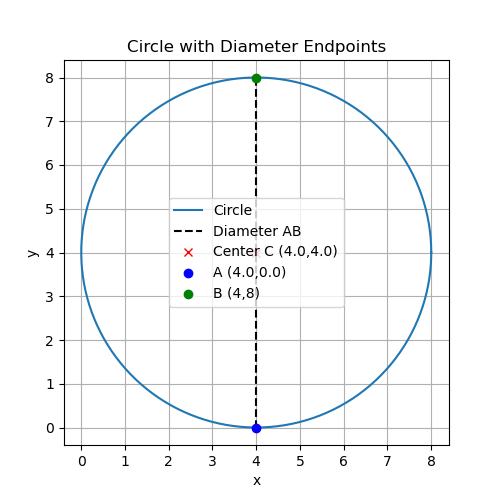
\includegraphics[width=0.7\textwidth, height=0.8\textheight]{figs/Figure_1.png}     
\end{frame}

\end{document}